\documentclass[12pt]{article}
\usepackage{amsmath}
\usepackage{graphicx}
\usepackage{subfigure}
\setlength{\oddsidemargin}{0.5in}
\setlength{\evensidemargin}{0.5in}
\setlength{\textwidth}{6.0in}
\setlength{\topmargin}{.75in}
\setlength{\textheight}{8.6in}


% Modified by S. Aubin for the 2018 mid-year reports

%
% This is a LaTeX template for an undergraduate mid-year report
%   in physics at William & Mary. Created from
%   several theses from previous students of D.S. Armstrong,
%   pared down to bare bones.
%
%   You will need this present file (MidyearReport_template.tex)
%   as well as the file figure1.pdf  to make the whole document

%  
%   For simplicity, we don't use bibtex here; experts can choose
%   to use that more powerful way of dealing with citations.
%

\begin{document}
\setlength{\baselineskip}{24pt}
\begin{titlepage}
\LARGE
\begin{center}
Mid-Year Report\\[2.3cm]

{\bf Defining condensates in low-dimensional spin models through the gradient flow}\\[2.3cm]

\normalsize

Stuart Thomas\\[2.5cm]
\end{center}
\normalsize
\begin{flushright}
%\hfill Accepted for Honors \\[.5cm]
\hfill \hrulefill \\
\hfill \hfill Advisor: Prof. Christopher Monahan \\[7.0cm]
%\hfill \hrulefill \\Prof. Richard P. Feynman \\[.6cm]
%\hfill \hrulefill \\Prof. Marie Curie \\[.6cm]
%\hfill \hrulefill \\Prof. Ernest J. Rutherford \\[.6cm]
\end{flushright}
\begin{center}
Department of Physics\\
College of William and Mary\\
Williamsburg, Virginia\\
November 2020
\end{center}
\end{titlepage}

\setlength{\topmargin}{0.0in}

\pagenumbering{roman}

\setcounter{page}{5}

\begin{abstract}

\indent
We study the the effect of operator smearing---defined as a local averaging of the field---on the $O(3)$ nonlinear $\sigma$ model, particularly analyzing renormalization properties. Specifically, we analyze the ``gradient flow,'' a gauge-invariant form of smearing which introduces a new dimension known as ``flow time.'' We perform Monte-Carlo simulations with the Metropolis algorithm and the Wolff cluster algorithm to numerically calculate correlation functions in small ($N\sim 32$) and mid-size ($N\sim128$) lattices, in 1+1 and 2+1 dimensions. To verify numerics, we first find the phase transition of scalar $\phi^4$ theory to be at $m_0^2=-0.72$ and $\lambda=0.5$, in agreement with previous literature.

\end{abstract}

\section{Introduction}
\pagenumbering{arabic}
\indent Lattice quantum chromodynamics (QCD) provides a method to explore and understand the strong nuclear force by discretizing spacetime. Specifically, lattice QCD can provide an understanding of nonperturbative theories which cannot be solved with traditional QFT techniques. With this technique, the path integrals that are key to quantum field theory become manageable and numerically calculable. When taking the lattice spacing to zero, which requires renormalizing all observables, we expect operators to remain finite, however this is not always the case. Some observables mix on the lattice, leading to divergencies. As an example, states of definite angular momentum mix when discretized. In our paper, we study power-divergent mixing, arising from the mixing of operators with different mass dimension. \cite{monahan2016}.

\subsection{Gradient Flow}

One technique to resolve this divergence is by ``smearing,'' a local averaging of a gauge field in order to remove diverging fluctuations \cite{solbrig2007}. Specifically, we use a technique known as ``gradient flow'' \cite{monahan2015} which introduces a new half-dimension called ``flow time''. The flow time parameterizes the smearing; an evolution in flow time corresponds to suppressing ultraviolet divergences. In a 2D $\phi^4$ scalar field theory, given by the action
\begin{equation}
    S_\phi [\phi] = \frac{1}{2}\int d^2x\left[(\partial \phi)^2+m^2\phi^2+\frac{\lambda}{2}\right],
\end{equation}
we can define the evolution in flow time as
\begin{equation}
    \frac{\partial \rho(\tau, x)}{\partial \tau} = \partial^2 \rho(\tau,x)
\end{equation}
where $\partial^2$ is the Laplacian in 4-D Euclidean spacetime and $\tau$ is the flow time. Here, $\rho$ is the field evolved into a nonzero flow time, bounded by the condition $\rho(\tau=0,x) = \phi(x)$. When solved exactly, this function forms a Gaussian which forces operators to converge. Therefore, in all orders of pertubation theory, any correlation function in the gauge field that has been evolved in flow time becomes immune to these divergences\cite{makino2015a}.

Generally, we can choose any flow time equation that drives the field towards a classical minimum. Beyond the $\phi^4$ model, we need flow equations that incorporate different types of fields. In the nonlinear $\sigma$ model, it has been shown that an appropriate manifestation of the flow time can resolve divergencies \cite{makino2015a}. Therefore, it is possible to define a different flow equation for this model as well. Our goal is to understand this renormalizability in the nonlinear $\sigma$ model using the gradient flow. Specifically, we seek to define vacuum condensates, or nonpertubative vacuum expectation values.

To explore this technique, we first plan to produce numerical calculations using a nonlinear $\sigma$ model. Using a Monte Carlo method in 1+1 dimensions, we can calculate the correlation functions of quantum field theories. With more computing power, expanding this simulation to 2+1 dimensions would provide an analysis more relevant to quantum chromodynamics.  Following this numerical calculation, we seek to find and understand an implementation of the gradient flow in this model using analytic methods. This understanding can then be verified by the numerical solution. 

\subsection{Field theories on the lattice}

The basis for lattice quantum field theory lies in the Feynman path integral formulation of quantum field theory. This formalism predicts the behavior of quantum fields using a ``path integral,'' or a integral of a function over all possible field configurations in space and time. Though nearly impossible to solve analytically, discretizing the field makes numerical solutions clear. Particularly, the correlation functions of the theory can be calculated using the generating functional, given as 
\begin{equation}
    Z[J] = \int \mathcal{D} \phi e^{iS[\phi]}
\end{equation}
where $\int \mathcal{D} \phi$ is a path integral over $\phi$ and $S$ is the action. We can apply a Wick rotation to the lattice to transform the Minkowski spacetime to Euclidean spacetime. This change of basis produces an alternative definition 
\begin{equation}
    Z[J] = \int \mathcal{D}\phi e^{-S_E[\phi]}
\end{equation}
where $S_E$ is the action in Euclidean space.

Theoretically, we could calculate every possible configuration of $\phi$ to obtain an exact value of $Z[J]$, but the computational time makes this method impossible. A more intelligent approach starts with noticing that significant contributions are relegated to the minimum of the action. Therefore, we can accurately determine the generating function, and also most relevant physics, by only considering contributions near the classical limit. However, determining which configurations to consider is nontrivial and is discussed in Section~\ref{sec:mc}.

In order to compare with existing literature, we first study the $\phi^4$ model, described by the action 
\begin{equation}
    S_E = \int d^D x \left[ \partial^\mu \phi \partial_\mu\phi + \frac{1}{2} m_0^2 \phi^2 + \frac{\lambda}{4}\phi^4\right]
\end{equation}
where $m_0^2$ and $\lambda$ are parameters of the theory. This model will provide a stepping stone for the vector-valued nonlinear $\sigma$ model.

\subsection{Non-linear $\sigma$ model}

The nonlinear $\sigma$ model is a prototypical theory for many physical phenomena, including applications in string theory. As a simple nonperturbative model, it provides an ideal starting point for lattice QCD studies. Specifically, the nonlinear $\sigma$ model exhibits many properties shared by Yang-Mills gauge theories, such as a mass gap, asymptotic freedom and $O(2)$ renormalizability. Furthermore, it has an exact application to Heisenberg ferromagnets in condensed matter. The theory is defined by the action 
\begin{equation}
    S_E = \frac{1}{2g^2} \int d^Dx \partial^\mu \vec\phi \cdot \partial_\mu \vec\phi
\end{equation}
subject to the constraint that $\vec\phi\cdot\vec\phi = 1$. In this report, we primarily consider $O(3)$, where $\vec\phi$ is a $3$ dimensional vector.

In order to use this theory on the lattice, we discretize the action. We replace the derivatives with a simple difference and impose periodic boundary conditions on the system.

\section{Computational Framework}
\label{sec:methods}
Our study of the gradient flow in the nonlinear $\sigma$ model consists of a computational part and an analytical part. We begin by outlining a numerical Monte Carlo method to simulate the lattice in 2 and 3 dimensions. We verify our program with the well-studied $\phi^4$ scalar field theory. Then, we plan to use this system to calculate twist-2 operators and vacuum expectation values in flow time, supporting a subsequent analytical study of such objects.

We implement these two algorithms first in Python for the $\phi^4$ model. Afterwards, we transition to C/C++ code due to the increased speed for more complicated theories. 

\subsection{Monte Carlo Simulations}
\label{sec:mc}

We implement a Markov Chain Monte Carlo method following Schaich's thesis \cite{schaich2006}. This implementation utilizes a ``random walk,'' i.e. a set of random steps through phase space, to determine statistical values such as correlation functions across the lattice. By the definition of the Markov chain, the probability of adoption of each state, and therefore its inclusion in the Monte Carlo calculation, depends only on the current state and the proposed state. This probability is denoted as $P(\mu\rightarrow\nu)$ where $\mu$ and $\nu$ are the existing and proposed lattice configurations respectively. We use a combination of the Metropolis and Wolff algorithms to determine this value.

\subsubsection{Metropolis Algorithm}
We primarily use the Metropolis algorithm for the calculation of new Markov chain configurations. We begin with a so-called ``hot start,'' where each field value at each lattice site is randomly selected. Then we propose a new value for a single lattice point, which is accepted with a probability
\begin{equation}
    P(\mu\rightarrow\nu) = \begin{cases} 
        e^{-(S_\nu - S_\mu)} & S_\nu > S_\mu \\
        1 & \mathrm{otherwise} \\
   \end{cases}
\end{equation}
where $S_\nu$ and $S_\mu$ are the lattice actions of configuration before and after the change. This process is performed for each point on the lattice, making up a ``sweep.'' Repeating this sweep many times pushes the lattice toward the action minimum.

\subsubsection{Wolff Cluster Algorithm}

Though the Metropolis algorithm will slowly find the absolute minimum of the theory, the presence of local minima can greatly prolong the convergence. Both the $\phi^4$ model and the nonlinear $\sigma$ model feature ``kinetic'' terms with gradients of $\phi$. Therefore, the presence of large similarly-valued regions in the lattice can lead to a local minimum. The Wolff algorithm helps reduce the presence of these clusters through two steps: identifying a cluster and flipping it along some arbitrary vector. In the case of $\phi^4$ theory, this flipping takes the form of a simple sign change. To identify the cluster, the algorithm uses a recursive algorithm defined by the probability of adding a new site. In the $\phi^4$ model, this takes the form of
\begin{equation}
    P_{add} = 1-e^{-2\phi_a\phi_b}.
\end{equation}


\subsubsection{Checkerboard algorithm}

In order to parallelize the Metropolis algorithm, we use a checkerboard algorithm. Since the Lagrangian density at each site does not depend on any sites diagonal to it, the lattice can be split into ``white'' sites and ``black'' sites, like the tiles on a checkerboard. Each white site is independent of every other white site and likewise with black sites. Therefore, we can split the sites of each color into separate parallel processing nodes and independently run the Metropolis algorithm, ensuring that no site affects the Lagrangian density at any other site. We use this method to parallelize the code through the Message Passing Interface (MPI).

\subsubsection{Autocorrelation times and thermalization}
One important aspect is the correlation between different states of the Markov chain. Ideally, each sample of the lattice would be completely independent, but this is not the case. Therefore, we must sweep the lattice sufficiently to produce an effective Monte Carlo result. We use Wolff's automatic windowing procedure \cite{wolff2007} and the $|\bar\phi|$ operator to estimate the autocorrelation and determine an appropriate number of sweep between measurements for each theory. Furthermore, the initial values of our Markov chain will be highly correlated with the initial random start. Therefore, we also wait a set number of sweeps before taking any measurements so that the lattice can approach a minimum of the action.


\section{Results}
We initially implemented the $\phi^4$ model using the Monte Carlo method described in Sec.~\ref{sec:methods} to verify the results of our system. According to previous studies (\cite{monahan2016}, \cite{schaich2006}), the $\phi^4$ model exhibits a symmetric and broken phase depending on its parameters $m_0^2$ and $\lambda$, specifically occurring at $m_0^2 = -0.72$ for $\lambda = 0.5$. We verify this result by plotting four observables: the lattice average $|\langle\bar\phi\rangle|$, the lattice variance $\chi$, the Binder cumulant $U$ and the bimodality $B$ in Fig.~\ref{fig:phi4}.

\begin{figure}[h]
  \centering
      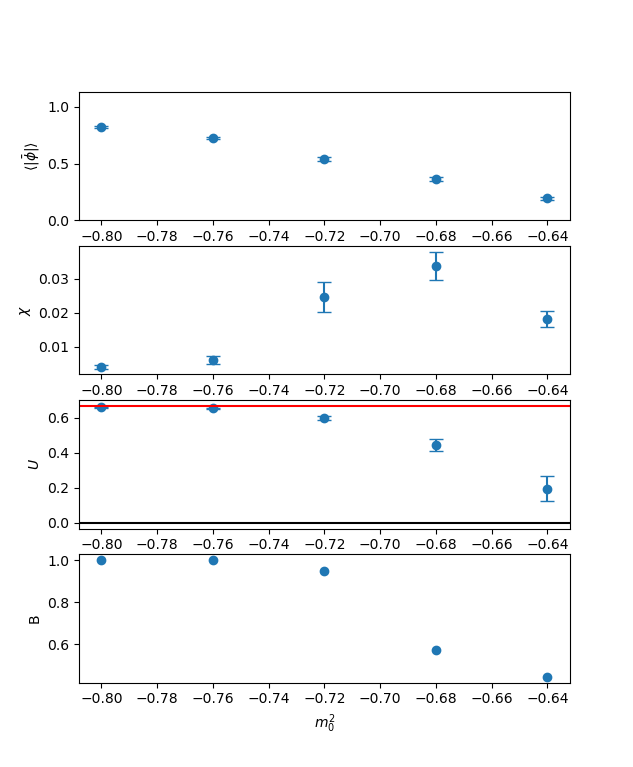
\includegraphics[width=0.7\textwidth]{imgs/phi4.png}
      \caption{The lattice average $|\langle\bar\phi\rangle|$, the lattice variance $\chi$, the Binder cumulant $U$ and the bimodality $B$ plotted as functions of $m_0^2$. $N=32$, $\lambda=0.5$. The lattice was thermalized from a hot start for 1000 sweeps. Afterwards, 100 measurements were taken with 100 sweeps between each. The red horizontal line indicates $U=2/3$, the symmetric limit of the Binder cumulant.}
  \label{fig:phi4}
\end{figure}

To improve efficiency, we transitioned from a Python based simulation to a C++ code. The comparison between these results are found in Fig.~\ref{fig:compare}, using the same values from Fig.~\ref{fig:phi4}.

\begin{figure}[h]
  \centering
      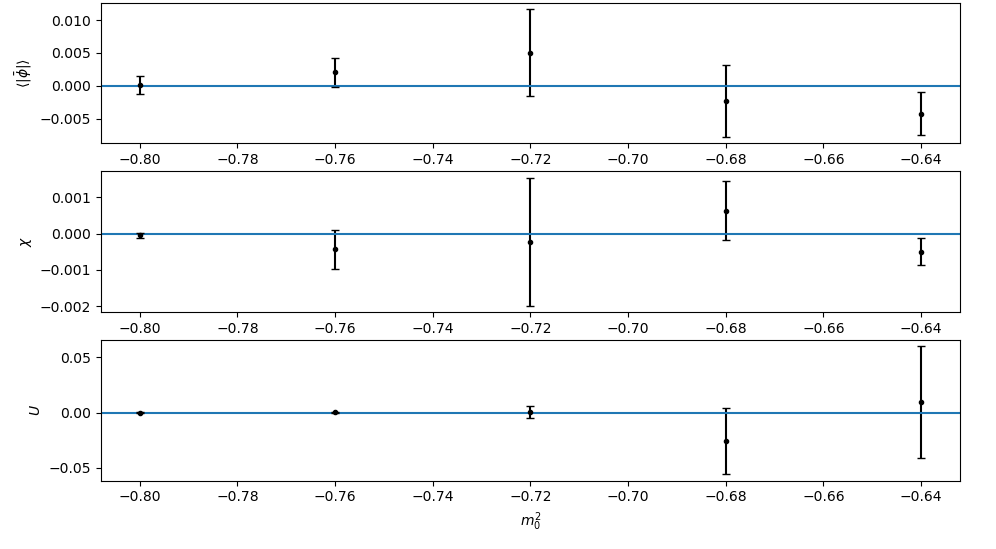
\includegraphics[width=0.7\textwidth]{imgs/compare.png}
      \caption{Comparison between Python and C++ code, using the lattice average $|\langle\bar\phi\rangle|$, the lattice variance $\chi$, the Binder cumulant $U$ and the bimodality $B$ plotted as functions of $m_0^2$. $N=32$, $\lambda=0.5$. The lattice was thermalized from a hot start for 1000 sweeps. Afterwards, 100 measurements were taken with 100 sweeps between each. The red horizontal line indicates $U=2/3$, the symmetric limit of the Binder cumulant.}
  \label{fig:compare}
\end{figure}


Furthermore, we implemented the gradient flow in this theory. Fig.~\ref{fig:flow} demonstrates the effect of the gradient flow on scalar lattice, specifically the dampening of high frequency modes.
\begin{figure}[h]
  \centering
      \subfigure[$\tau=0$]{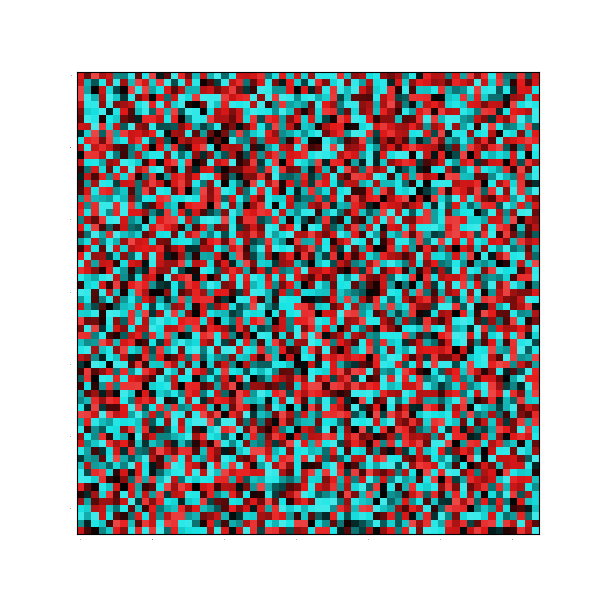
\includegraphics[width=0.20\textwidth]{imgs/0.png}}
      \subfigure[$\tau=0.5$]{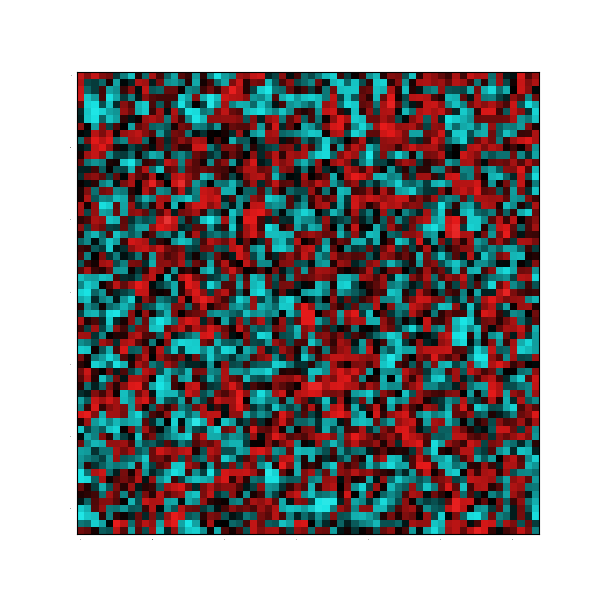
\includegraphics[width=0.20\textwidth]{imgs/0_5.png}}
      \subfigure[$\tau=2$]{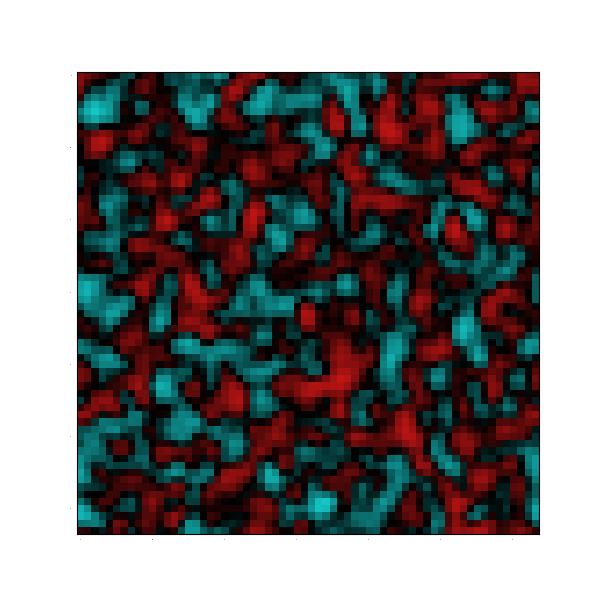
\includegraphics[width=0.20\textwidth]{imgs/2.png}} 
      \subfigure[$\tau=10$]{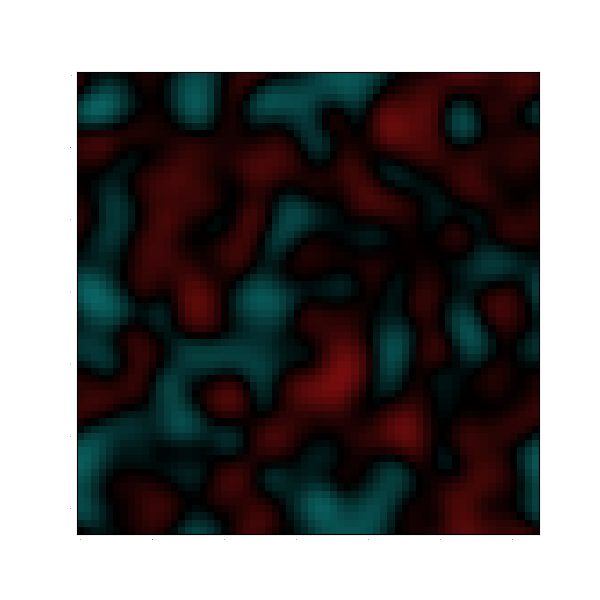
\includegraphics[width=0.20\textwidth]{imgs/10.png}}
          \caption{Effect of flow time evolution on a random lattice in the symmetric phase. Red and blue indicate positive and negative values of the field in 2D spacetime.}
  \label{fig:flow}
\end{figure}

\section{Future work}
All of our current results apply only to the $\phi^4$ theory. Therefore, our future work primarily includes completing the migration to the nonlinear $\sigma$ model implemented in C/C++. Afterwards, we plan on analyzing the effect of the gradient flow numerically. Finally, we plan to use analytical techniques to understand the numerical results.

Our main numerical result will be the vacuum expectation values of operators, which we will use to define condensates in the nonlinear $\sigma$ model. These condensates are vital for understanding the physical make-up of hadrons and therefore would be valuable to the field of QCD. We also may consider topological states on the lattice.

\begin{flushleft}
\bibliographystyle{unsrt}
\bibliography{midyear-report}
%\begin{thebibliography}{99.}

%\bibitem{Perkins} Perkins, Donald H.  Introduction to High Energy
%Physics.  3rd ed.  Menlo Park: Addison-Wesley, 1987.

%\bibitem{Perkins} Perkins, Donald H.  Introduction to High Energy
%Physics.  3rd ed.  Menlo Park: Addison-Wesley, 1987.

%\bibitem{IsgurKumano} F. Close, N. Isgur and S. Kumano,
%Nucl. Phys. {\bf B389}, 513 (1993).

%\bibitem{UPV} Alex Dubanowitz, Senior project thesis, College of
%William and Mary, 1998. (unpublished).



%\end{thebibliography}
\end{flushleft}

\end{document}
